% !TEX program = xelatex
%% Requires compilation with XeLaTeX or LuaLaTeX
\documentclass[10pt,xcolor={table,dvipsnames},t]{beamer}
\usepackage{biblatex}
\usepackage{caption}
\setbeamertemplate{caption}[numbered]
\addbibresource{reference.bib}
\usepackage{hyperref}
\hypersetup{ 
pdfpagemode=FullScreen,  
colorlinks=true,linkcolor=blue}
\usepackage{enumerate}

\usepackage{listings}
\usepackage{xcolor}

\definecolor{codegreen}{rgb}{0,0.6,0}
\definecolor{codegray}{rgb}{0.5,0.5,0.5}
\definecolor{codepurple}{rgb}{0.58,0,0.82}
\definecolor{backcolour}{rgb}{0.95,0.95,0.92}

\lstdefinestyle{mystyle}{
    backgroundcolor=\color{backcolour},   
    commentstyle=\color{codegreen},
    keywordstyle=\color{magenta},
    numberstyle=\tiny\color{codegray},
    stringstyle=\color{codepurple},
    basicstyle=\ttfamily\footnotesize,
    breakatwhitespace=false,         
    breaklines=true,                 
    captionpos=b,                    
    keepspaces=true,                 
    numbers=left,                    
    numbersep=5pt,                  
    showspaces=false,                
    showstringspaces=false,
    showtabs=false,                  
    tabsize=2
}

\lstset{style=mystyle}

% Flow chart config
\usepackage{tikz}
\usetikzlibrary{calc,trees,positioning,arrows,fit,shapes,calc}
\usetikzlibrary{shapes.geometric, arrows}
\tikzstyle{startstop} = [rectangle, rounded corners, minimum width=3cm, minimum height=1cm,text centered, draw=black, fill=red!30]
\tikzstyle{io} = [trapezium, trapezium left angle=70, trapezium right angle=110, minimum width=3cm, minimum height=1cm, text centered, draw=black, fill=blue!30]
\tikzstyle{process} = [rectangle, minimum width=3cm, minimum height=1cm, text centered, draw=black, fill=orange!30]
\tikzstyle{decision} = [diamond, minimum width=3cm, minimum height=1cm, text centered, draw=black, fill=green!30]
\tikzstyle{arrow} = [thick,->,>=stealth]

\usetheme{UCBerkeley}

\title[Your Short Title]{STMC HKOI Training}
\subtitle{Mathematical Proofs}
\author{Chan Yan Mong}
%\institute{}
\date{\today}

\begin{document}

\begin{frame}
  \titlepage
\end{frame}

% Uncomment these lines for an automatically generated outline.
%\begin{frame}{Outline}
%  \tableofcontents
%\end{frame}

\section{Class Goal}

\begin{frame}{Goal today}

\begin{itemize}
  \item Proof in mathematics
  \item Implication 
  \item Contrapositive
  \item Contradiction
  \item Mathematical Induction
\end{itemize}

\end{frame}


\section{Proof in mathematics}
\begin{frame}{Mathematics is not arithmetic}
    \begin{itemize}
      \item What does it mean to be good in mathematics?
      \item Are mathematicians human-calculators?
      \item In fact, mathematics is different from arithmetic, the computation of numbers
    \end{itemize}
\end{frame}

\begin{frame}{Example: Sum of odd numbers}
  Consider the following sum:
  \begin{align*}
    S=1 + 3 + 5 + 7 + \cdots + 99
  \end{align*}
  What is the value of the sum?
\end{frame}

\begin{frame}{Example: Sum of odd numbers}
  \begin{itemize}
    \item Someone who are reluctant to think will simply crunch the numbers and calculate the sum term by term (arithmetic)
    \item However, a mathematician would look for \textit{patterns} in the sum
    \item Let's embark on a journy to enhanace our problem solving skills and be more like a thinker, but not a calculator
  \end{itemize}
\end{frame}

\begin{frame}{Example: Sum of odd numbers}
  \begin{itemize}
    \item A very useful strategy in problem solving in general is to \textbf{list a few special cases}:
  \end{itemize}
  \begin{table}
    \centering
    \begin{tabular}{|c|r|}
      \hline $n$ & $S$\\\hline
      1 & 1\\
      2 & 1+3=4\\
      3 & 1+3+5=9\\
      4 & 1+3+5+7=16\\
      5 & 1+3+5+7+9=25\\\hline
    \end{tabular}
  \end{table}
  Did you spot a pattern?
\end{frame}

\begin{frame}{Example: Sum of odd numbers}
  \begin{itemize}
    \item According to our observation, it seems like the sum of first $n$ odd numbers is $n^2$
    \item Therefore we form a \textbf{hypothesis}:
    \begin{exampleblock}{Hypothesis:}
      \begin{center}
        \textit{The sum of first $n$ odd numbers is $n^2$}
      \end{center}
    \end{exampleblock}
    \item \textit{If} this hypothesis is true, then we can immediately get the answer, because 99 is the 50th odd number, so the answer is simply $50^2 = 2500$
    \item \textit{But is it?} Before answering the question, let's look at the story of Gauss
  \end{itemize}
\end{frame}

\begin{frame}{Carl Friedrich Gauss}
  \begin{columns}
    \begin{column}[T]{0.7\textwidth}
    \setlength{\partopsep}{0pt}
    \textbf{Carl Friedrich Gauss} is one of the greatest mathematician in history. Often termed as the "Prince of Mathematics", he made exceptional contributions across many fields in mathematics and science.

    \vspace{0.6cm}
    Today, we shall look at a widely circulated story of his early genius and reflect on important elements of mathematical thinking along the way.
    \end{column}
    \begin{column}[T]{0.3\textwidth}
        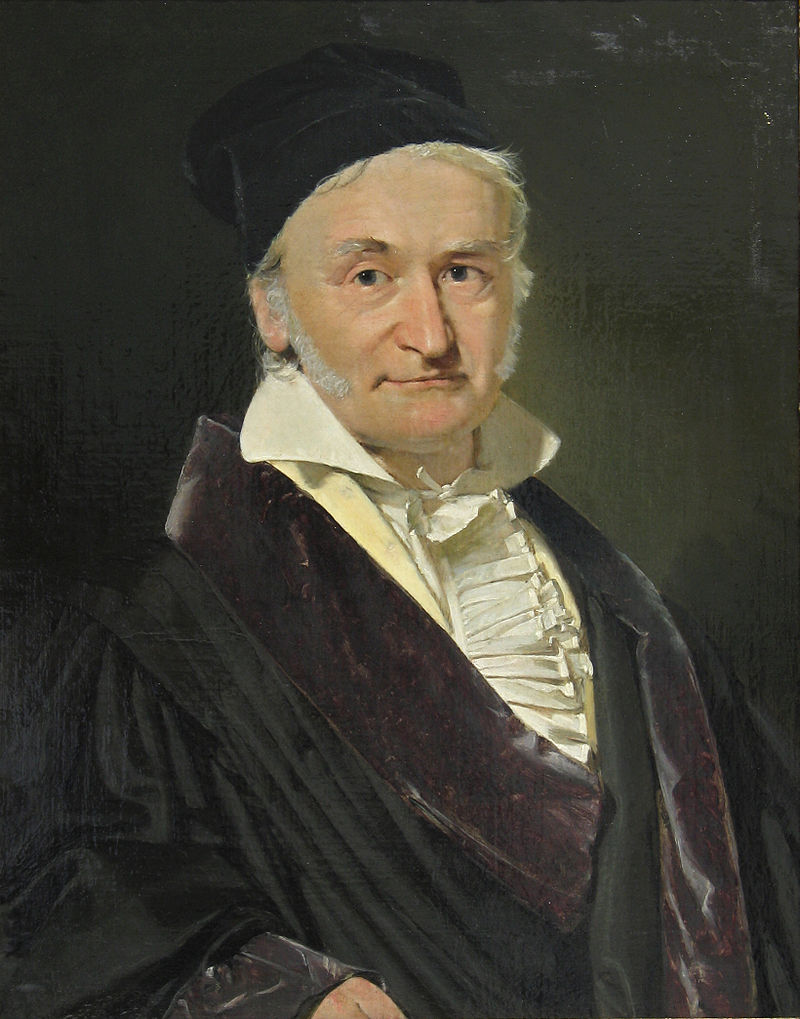
\includegraphics[width=\textwidth]{img/gauss.jpg}

    \end{column}
  \end{columns}
\end{frame}

\begin{frame}{Story about summing from 0 to 100}
  This version of the story is adapted from \href{https://nrich.maths.org/2478}{NRICH}
  \begin{itemize}
    \item When Gauss was still at primary school, his teacher one day told asked his class to add together all the numbers from $1-100$, assuming that this task would occupy them for quite a while. 
    \item However, to the shock of his teacher, Gauss quickly found the correct answer: $5050$
  \end{itemize}
  \begin{align*}
    1 + 2 + 3 + \cdots + 100 = 5050 
  \end{align*}
\end{frame}

\begin{frame}{Story about summing from 0 to 100}
  \begin{itemize}
    \item How did he do it? Eight year old Gauss pointed out that the problem was actually quite simple.
    \item What he observed is as follows:
  \end{itemize}
  \begin{align*}
    S &= 1 + 2 + 3 + \cdots + 98 + 99 + 100\\
    S &= 100 + 99 + 98 + \cdots + 3 + 2 + 1\\
    \therefore 2S &= (1+100) + (2+99) \cdots+ (99+2) + (100+1)\\
    &= (101) + (101) + \cdots + (101) + (101) = 101\times 100\\
   \therefore S & = 101 \times 50 = 5050
  \end{align*}
\end{frame}

\begin{frame}{Story about summing from 0 to 100}
  \begin{itemize}
    \item What did we learn in this story?
    \item This story tells us that rather than blindly performing mental arithmetic, \textbf{a clean solution can be found by exploiting the structure of the problem}
    \item Furthermore, by investigating the structure, we in turns \textbf{gain more insight than headless computation}
    \item In fact, this is the difference between arithemtic and mathematics
  \end{itemize}
\end{frame}

\begin{frame}{Going back to the sum of odds ...}
  \begin{itemize}
    \item<1-> Can you now provide an logical argument why the sum of first $n$ odd numbers is $n^2$?
    \item<2> Here is a solution
  \end{itemize}
  \begin{align*}
    \uncover<2>{S &= 1 + 3 + 5 + \cdots + 2n-1\\
    S &= 2n-1 + 2n-3 + \cdots  + 1\\
    \therefore 2S &= (2n) + (2n) + \cdots + (2n)= 2n^2\\
    \therefore S &= n^2} 
  \end{align*}
\end{frame}

\begin{frame}{Short summary}
  Hopefully, through this example, you see that: 
  \begin{itemize}
    \item The greatest insight always lies in discovering the \textit{structure} of the problem
    \item Examples can reveals structure within a problem
    \item You have to \textit{provide an argument (proof)} to support your hypothesis
  \end{itemize}
\end{frame}

\section{Importance of proof}
\begin{frame}{Importance of proof}
  \begin{itemize}
    \item In the summary above, we have stressed the importance of providing a proof / argument to support your claim
    \item Curious of you may wonder: Why all the trouble? After all, if something holds for many situation, wouldn't it holds for all situation?
    \item The short answer is no. \textbf{Unless we enumerate all possibilities, things that holds true for large number of cases can fail}
  \end{itemize}
\end{frame}

\begin{frame}{Importance of proof}
  \begin{itemize}
    \item To see the point, let's consider a famous example.
    \item Consider the following sequence by Euler (1774):
    \begin{align*}
      F_n = n^2 - n + 41
    \end{align*}
    \item If we list the put $n=0,1,2,3,\cdots, 39, 40$ to the sequence, we will found that all of them are prime numbers (Try it!)
    \item However, when $n=41$ $F_{41}$ is obviously not a prime because $F_{41} = 1681 = 41^2$ 
  \end{itemize}
\end{frame}

\begin{frame}{Importance of proof}
  Some terms of $F_n$:
  \begin{table}[]
    \begin{tabular}{llllllllllll}
    $n$   & 1  & 2  & 3  & 4  & 5  & $\cdots$ & 37   & 38   & 39   & 40   & 41   \\
    $F_n$ & 41 & 43 & 47 & 53 & 61 & $\cdots$ & 1373 & 1447 & 1523 & 1601 & \textcolor{red}{1681}
    \end{tabular}
    \end{table}
  From $n=1-40$, $F_n$ are all primes, but when $n=41$ it fails. This illustrated something that holds true for a large number of cases won't necessarily holds forever.

  \vspace{0.5cm}

  Therefore, we need always need to find a \textbf{proof} to demonstrate results definitively.
\end{frame}

\section{Implication}
\begin{frame}{Implication}
  \begin{itemize}
    \item Let $P$,$Q$ be two statements. When say \textbf{P implies Q} or \textbf{If P then Q}, we mean:
    \begin{center}
      \textit{"If $P$ is true, then $Q$ is true"}
    \end{center}
    \item For example, when we say \textit{"If the sky is cloudy, the sun is not visible"}. We have:
    \begin{align*}
      P &= \text{The sky is cloudy}\\
      Q &= \text{The sun is not visible}\\
      P\implies Q &= \text{If the sky is cloudy, then the sun is not visible}
    \end{align*}
  \end{itemize}
\end{frame}

\begin{frame}{Implication}
  \begin{itemize}
    \item Note that when $P$ is false, $Q$ can be either true or false. For example, even when the sky is not cloudy, it doesn't mean that the sun is visible, it can as well be that it's midnight.
    \begin{center}
      Sky not cloudy $\;\not\!\!\!\implies$ Sun is visible
    \end{center}
    \item In a similar vein, $P\implies Q$ \textbf{does not imply} $Q\implies P$. A simple counterexampe: If someone is your father, he is a male. But that does not imply if someone is a male, he is your father.
  \end{itemize}
\end{frame}

\begin{frame}{Implication}
  \begin{itemize}
    \item Some more examples showing that $P\implies Q$ does not mean $Q\implies P$:
    \begin{enumerate}
      \item If a shape is a square, it has 4 right angles $\;\not\!\!\!\implies$ If a shape has 4 right angles, it is a square
      \item If a number is divisible by 4, it's divisible by 2 $\;\not\!\!\!\implies$ If a number is divisible by 2, it's divisible by 4
      \item If $x$ is positive, $x^2$ is positive $\;\not\!\!\!\implies$ If $x^2$ is positive, $x$ is positive
      \item If you are sad, you cry $\;\not\!\!\!\implies$ If you cry, you are sad
    \end{enumerate}
    \item Hopefully these examples are enough to convince you that proving "if A then B" and "if B then A" are different things
  \end{itemize}
\end{frame}

\begin{frame}{Exercise}
  Let's prove the following statements:
  \begin{enumerate}
    \item Let $a,b$ be two positive integers, if $a$ is odd and $b$ is even, then $a+b$ is odd (Hint: A odd number can alway be written in form of $2n+1$) 
    \item If $n$ is odd, then $3n+5$ is even
    \item If $n$ is odd, then $4n^3 + 2n+1$ is odd
    \item If $b,c$ are divisible by $a$, then $bc$ is divisible by $a$
  \end{enumerate}
\end{frame}

\section{Contradiction}
\begin{frame}{Proof by Contradiction}
  \begin{itemize}
    \item Now we shall introduce some proving techniques. On of such techniques is called \textbf{proof by contradiction}
    \item Let's consider an example: 
  \end{itemize}
  \begin{exampleblock}{Example:}
    If $x^2$ is divisible by 2, then $x$ is divisible by 2.
    \begin{proof}
      Suppose it's wrong and there exist some $x_0$ so that $x_0^2$ is even but $x_0$ is odd. Then since $x_0$ is odd, $x_0 = 2n+1$. But that implies $x_0^2 = (2n+1)^2 = 4n^2 + 4n + 1$ $= 2(2n+2) + 1$, which is odd. But $x_0^2$ cannot be odd and even, so contradiction.
    \end{proof}
  \end{exampleblock}
\end{frame}

\begin{frame}{Proof by Contradiction}
  \begin{itemize}
    \item As illustrated in the example, a proof by contradiction works by assuming the statement is wrong, then derive a contradiction, that is, an impossible situation from the assumption, which disprove the assumption and proves the original statement.
    \item Let's demonstrate that with another example.
  \end{itemize}
\end{frame}

\begin{frame}{Proof by Contradiction}
  \begin{exampleblock}{Statement}
    There exist no integers $a,b$ for which $18a+6b=1$
    \begin{proof}
      Suppose not, that is, there exist some integers $a,b$ so that $18a+6b=1$, then divide both side by $6$, we have $3a+b=1/6$, but this is impossible, because the LHS is an integer by RHS is not. So a contradiction is reached. Hence there does not exist integers $a,b$ for which $18a+6b=1$
    \end{proof}
  \end{exampleblock}
\end{frame}

\begin{frame}{Exercise}
  Here are some exercises:
  \begin{enumerate}
    \item If two integers $a,b$ satisfy $a+b\geq 19$, then $a\geq 10$ or $b\geq 10$
    \item If $a^2-2a+7$ is even then $a$ is odd
    \item If $a$ is a real number, then $a^2 \geq 0$
    \item If $ab=0$ then either $a$ or $b$ equals to 0
    \item If $a,b$ are integers, then $a^2-4b-2\neq 0$
    \item Suppose $a,b,c$ are integers and $a^2 + b^2 = c^2$, then $a$ or $b$ is even
  \end{enumerate}
\end{frame}

\section{Contrapositive}
\begin{frame}{Proof by Contrapositive}
  \begin{itemize}
    \item As we have illustrated in previous examples $P \implies Q$ does not mean $Q\implies P$.
    \item However, we can show that if $P \implies Q$, then $\text{not}\,Q \implies \text{not}\,P$
  \end{itemize}
  \begin{theorem}[Contrapositive]
    If $P \implies Q$, then $\text{not}\,Q \implies \text{not}\,P$
    \begin{proof}
      We shall use contradiction. Suppose $P \implies Q$ is true but somehow  $\text{not}\,Q \implies \text{not}\,P$ is false. Then for some $P,Q$ we have $Q$ is false but $P$ is true. But by assumption, $P\implies Q$, so $Q$ must be true, which is a contradiction.
    \end{proof}
  \end{theorem}
\end{frame}


\begin{frame}{Proof by Contrapositive}
  \begin{itemize}
    \item The result provide the grounding for a method of proof called \textbf{proof by contrapositive}
    \item In short, because $p \rightarrow q$ is equivalent to $\neg q \rightarrow \neg p$, we can prove a statement by it's contrapositive, which is sometimes easier
    \item Consider the following claim:
    \item \textbf{Claim:}
      Let $x\in\mathbb{Z}^+$. If $x^2 -6x + 5$ is even, then $x$ is odd.
    \item How can we prove this claim?
  \end{itemize}
\end{frame}
\begin{frame}{Proof by Contrapositive}
  \begin{itemize}
    \item Instead proving directly, we prove it's contrapositive. 
    \item The contrapositive of the statement is:
    \item \textbf{Contrapositive Claim:} If $x$ is even, then $x^2 - 6x + 5$ is odd
    \item This is almost trivial to prove, because:
    \begin{align*}
      x^2 - 6x + 5 = \overbrace{x(x-6)}^{\text{even if x even}} + \overbrace{5}^{\text{odd}}
    \end{align*}
    So the sum must be odd
  \end{itemize}
\end{frame}


\section{Mathematical induction}
\begin{frame}{Mathematical induction}
  \begin{itemize}
    \item We shall introduce a proving technique which we will use very often in the future
    \item This is called the \textbf{mathematical induction}
    \item This method is very useful in proving statement of form $P(n)$, with $n$ being positive integers. Examples of such statements are:
    \begin{enumerate}
      \item "$1+2+3+\cdots + n = n(n+1)/2$ for all positive integer $n$"
      \item "For integer $n\geq 12$, there exist some integers $a,b$ such that $n=4a+5b$"
      \item "$3^n-1$ is a multiple of $2$ for $n=1,2,3,\cdots$"
    \end{enumerate}
    \item Let's try to introduce the idea with some example
  \end{itemize}
\end{frame}

\begin{frame}{Mathematical induction}
  \begin{exampleblock}{Example}
    Prove that $P(n)=1+2+3+\cdots + n = n(n+1)/2$ is true for $n \in \mathbb{Z}^+$
    \begin{proof}
      We will first prove that the statement is true when $n=1$:\\
      When $n=1$, LHS=$1$, RHS=$1(1+1)/2=1$. So it's true.\\
      Now \textbf{assume} $1+2+3+\cdots + k = k(k+1)/2$ for some integer $k$. We want to show $P(k)\implies P(k+1)$.This is easy, because if we know $P(k)$ is true, then RHS$=1+2+3+\cdots + k + k+1 = (1+2+3+\cdots + k) + k+1 = k(k+1)/2 + k+1 = (k+1)(k+2)/2=$LHS. So if $P(k)$ is true then $P(k+1)$ is true. But we have proved $P(1)$ is true. So $P(1)\implies P(2)$ and $P(2)\implies P(3)$ and so on. So we have successfully proved the statement is true for all $n$  
    \end{proof}
  \end{exampleblock}
\end{frame}

\begin{frame}{Mathematical induction}
  \begin{itemize}
    \item The example above illustrated the idea of mathematical induction
    \item In a mathematical induction proof, we first show that the statement holds for some simple cases (e.g. $n=1$). This is also called the \textbf{base case}.
    \item Then we show that if the statement is true for some integer $k$, then the statement is also true for the next integer $k+1$ (i.e. $P(k)\implies P(k+1)$). This is called the \textbf{induction step}
    \item Using the induction step repeatedly, we can show that the statement holds for all natural number $n$. 
    \item For example, if the base case is $P(1)$, and we show that $P(k)\implies P(k+1)$. Then $P(2)$ is true because $P(1)\implies P(1+1)$. But now $P(3)$ is also true because $P(2)\implies P(2+1)$. Repeating this we can show $P$ holds for all $n\geq 1$
  \end{itemize}
\end{frame}

\begin{frame}{Mathematical induction}
  \begin{exampleblock}{Example (Sum of squares):}
    Prove that:
    \begin{align*}
      1^2 + 2^2 + 3^2 + \cdots + n^2 = \frac{n(n+1)(2n+1)}{6}
    \end{align*}
    for all $n\geq 1$, $n$ is integer using mathematical induction.
  \end{exampleblock}
\end{frame}
\begin{frame}{Mathematical induction}
  \begin{proof}
    \only<1>{\textbf{Base case}: When $n=1$, LHS = $1^2 = 1$. RHS = $1(1+1)(2(1)+1)/6 = 1$. So $P(1)$ is true.\\
    \textbf{Induction step}: Suppose $P(k)$ is true, that is:
    \begin{align*}
      1^2 + 2^2 + \cdots + k^2 = \frac{k(k+1)(2k+1)}{6}
    \end{align*}}
    \only<2>{Then when $P(k+1)$:
    \begin{align*}
      \text{LHS}&=1^2 + 2^2 + 3^2 + \cdots k^2 + (k+1)^2\\
      &= \frac{k(k+1)(2k+1)}{6} + (k+1)^2\\
      &= \frac{\left[k(2k+1)+6(k+1)\right](k+1)}{6}\\
      &= \frac{(k+1)(k+2(2k+3)}{6} = \text{RHS}
    \end{align*}
    So by principle of mathematical induction the statement is true for all $n\geq 1$}
    
    \alt<2>{\qedhere}{\phantom\qedhere}
  \end{proof}
\end{frame}

\begin{frame}{Mathematical induction}
  \begin{exampleblock}{Example (Divisibility)}
    Show that $3^n-1$ is divisible by 2 for $n=1,2,3,\cdots$
  \end{exampleblock}
  \begin{proof}
    \textbf{Base case}: Trivial, because LHS=$3^1-1=2$ which is obviously divisible by 2.\\
    \textbf{Induction step}: If $3^k-1$ is divisible by 2 for some $k \in \mathbb{Z}^+$, then when $n=k+1$:
    \begin{align*}
      \text{LHS} &= 3^{k+1} - 1 = 3(3^{k}-1+1)-1 \\
      &= 3(3^{k}-1)+ 2 = 3(2N) + 2 = 2(3N + 1)
    \end{align*}
    which is obviously divisible by 2
  \end{proof}
\end{frame}

\begin{frame}{Mathematical induction}
  \begin{exampleblock}{Example (Checkerboard filling)}
    Prove that for any checkerboard of size $2^n\times 2^n$ can be tiled with L-shaped tiles in such a way that there is exactly one $1x1$ left anywhere we like in the checkerboard.
    \begin{proof}
      Refer to \url{https://www.amsi.org.au/teacher_modules/pdfs/Maths_delivers/Induction5.pdf} for the illustrations and proof.
    \end{proof}
  \end{exampleblock}
\end{frame}

\begin{frame}{Exercise}
  \begin{enumerate}
    \item Prove that $1^3 + 2 ^3 + 3^3 + \cdots + n^3 = \left[n(n+1)/2\right]^2$
    \item Show that $a+ar+ar^2 + \cdots + ar^{n-2}+ar^{n-1} = a(1-r^n)/(1-r)$
    \item Prove that $2^n \geq n$ for $n=1,2,3,\cdots$
    \item Prove that any integer $n\geq 2$ is either a prime or can be expressed as a product of primes
    \item A country has $n$ city, every city is connected by a one-way road. Show that there is a route that passes through every city.
  \end{enumerate}
\end{frame}

\end{document}
